\documentclass[10pt]{article}

\input{/Users/gabesekeres/Dropbox/LaTeX_Docs/pset_preamble.tex}

\course{ECON 6140}
\pset{1}
\begin{document}
\maketitle

\section*{Skill-biased technical change}

\begin{enumerate}
	\item The elasticity of substitution between capital $k_t$ and skilled labor $n_s$ is defined by:\[\frac{d \ln(k_t / n_s)}{d \ln (\text{MRS}_{sk})} \]where the marginal rate of substitution is \[\text{MRS}_{sk} = \frac{f_{n_s}(z,k_t,n_t)}{f_{k_t}(z,k_t,n_t)} = \frac{\mu n_s^{\rho-1}}{(1-\mu)k_t^{\rho - 1}} = \frac{\mu}{1-\mu} \frac{k_t^{1-\rho}}{n_s^{1-\rho}}\]which means that\[\ln(\text{MRS}_{sk}) = \ln\parl \frac{\mu}{1-\mu}\parr + (1-\rho) \ln\parl\frac{k_t}{n_s}\parr\] so we have that\[\frac{d\ln(\text{MRS}_{sk})}{d\ln(k_t/n_s)} = 1-\rho \Longrightarrow \frac{d \ln(k_t / n_s)}{d \ln (\text{MRS}_{sk})} = \frac{1}{1-\rho}\]The elasticity of substitution is constant, and dependent only on the parameter $\rho$.
	\item Recall that a steady state must satisfy the first order necessary conditions in the model for it to be interior (rather than the trivial steady state of 0 consumption). Our Lagrangian is \[\mathcal{L} = \sum_{t=0}^\infty \beta^t \curll u(c_t,1-n_t) + \lambda_t\barl f(z,k_t,n_t) - c_t - x_{k_t}\barr + \theta_t \barl (1-\delta_k)k_t + x_{k_t} - k_{t+1}\barr + \gamma_{1t}c_t + \gamma_{2t}n_t + \gamma_{3t}k_{t+1} \curlr\](along with non-negativity constraints and complementary slackness conditions) our first order conditions are \begin{align*} 0 &= u_c(c_t,1-n_t) - \lambda_t +\gamma_{1t} &&(c_t) \\ 0 &= -u_n(c_t,1-n_t) +\lambda_t f_n(z,k_t,n_t)+ \gamma_{2t} &&(n_t)\\ 0 &= -\theta_t + \beta \barl\lambda_{t+1} f_k(z,k_{t+1},n_{t+1}) + \theta_{t+1}(1-\delta_k)\barr + \gamma_{3t} &&(k_{t+1}) \\ 0 &= -\lambda_t + \theta_t &&(x_{k_t})\\ 0 &= \lim_{T\to\infty} \beta^T \lambda_T k_{T+1} &&(TVC) \\ f(z,k_t,n_t) &= c_t + x_{k_t} &&(\text{Feasibility})\end{align*} Using complimentary slackness and interiority, and simplifying, these become \begin{align*} u_c(c_t,1-n_t)&= \lambda_t \\ \lambda_t &= \lambda_{t+1} \beta \barl f_k(z,k_{t+1},n_{t+1}) + (1-\delta_k)\barr \\f(z,k_t,n_t) &= c_t + x_{k_t} \end{align*} If a steady state exists, it must satisfy these model equations -- we must have that it satisfies the Euler equation: \[ u_c(c\opt,1-n\opt) = u_c(c\opt,1-n\opt) \beta \barl f_k(z,k\opt,n\opt) + (1-\delta_k)\barr \Longrightarrow 1 = \beta \barl f_k(z,k\opt,n\opt) + (1-\delta_k)\barr\]It must also satisfy feasibility: \[f(z,k\opt,n\opt) = c\opt + x\opt \underbrace{\Longrightarrow}_{\text{LoM of }k} f(z,k\opt,n\opt) = c\opt + \delta k\opt \] For the Euler equation, it is necessary that $f_k(\cdot)$ be continuous, and also that the standard assumptions be true: \begin{align*} \lim_{k_t\to 0} f_k(\cdot) &> \frac{1}{\beta} - 1 + \delta \\ \lim_{k_t\to \infty} f_k(\cdot) &< \frac{1}{\beta} - 1 + \delta \end{align*} If all of these conditions hold, a steady state will necessarily exist.
	\item The skill premium is characterized as the ratio of the skilled wage $w_s$ to the unskilled wage $w_u$, which are the marginal products of skilled and unskilled workers respectively: \[w_u = \frac{\partial f}{\partial n_u} = z \parl \lambda(\mu (k_t)^\rho + (1-\mu)(n_s)^\rho)^{\frac{\sigma}{\rho}}+ (1-\lambda)n_u^\sigma\parr^\frac{1-\sigma}{\sigma} (1-\lambda)n_u^{\sigma-1}\]\[w_s = \frac{\partial f}{\partial n_s} = z\parl \lambda(\mu (k_t)^\rho + (1-\mu)(n_s)^\rho)^{\frac{\sigma}{\rho}}+ (1-\lambda)n_u^\sigma\parr^\frac{1-\sigma}{\sigma} \lambda(\mu(k_t)^\rho + (1-\mu)(n_s)^\rho)^\frac{\sigma - \rho}{\rho}(1-\mu)n_s^{\rho - 1}\]so the skill premium is \[\frac{w_s}{w_u} = \frac{\lambda}{1-\lambda}\frac{n_s^{\rho-1}}{n_u^{\sigma-1}} (1-\mu)(\mu(k_t)^\rho + (1-\mu)(n_s)^\rho)^\frac{\sigma - \rho}{\rho}\]
	\item We have that countries differ in productivity $z$. If every country is in steady state, capital accumulation satisfies \[k = \frac{x_k}{\delta_k} = \frac{f(z,k,n) - c}{\delta_k} \Longrightarrow \frac{k}{n_s} = \frac{f(z,k,n) - c}{n_s\delta_k} \]so a country with higher $z$ will have a higher capital / skill ratio, as $f$ is increasing in $z$. Similarly, output per worker is defined by \[\frac{y}{n} = \frac{f(z,k,n)}{n}\]which is also increasing in $z$, so a country with higher productivity will have a higher output per worker. Finally, we have an equation for the skill premium above, and we can directly see that it is not affected by $z$, so it will be the same across countries with different productivities.
	\item We now assume that countries differ in the ratio of skilled to unskilled workers $\frac{n_u}{n_s}$. As above, capital accumulation satisfies  \[k = \frac{x_k}{\delta_k} = \frac{f(z,k,n) - c}{\delta_k} \Longrightarrow \frac{k}{n_s} = \frac{f(z,k,n) - c}{n_s\delta_k} \]so a country with a higher ratio of unskilled workers to skilled workers will have an increase in the marginal productivity to skilled labor (because the relative decrease in supply of skilled workers) which will lead to a decrease in the capital to skilled labor ratio, as they will demand more skilled labor. When the ratio of unskilled workers to skilled workers increases, output per worker will decrease because a higher proportion of unskilled workers will decrease $f(\cdot)$ in steady state. Finally, in our equation for the skill premium above, we can see that a greater proportion of unskilled workers will increase the skill premium, as the (relative) marginal product of skilled workers will increase.
	\item As new technology appears, skill-biased technological change predicts that it will favor skilled workers over unskilled workers. In our model, we can see that the marginal product of skilled workers is increasing in $z$, as is the marginal product of unskilled workers. However, as long as the skill premium is greater than 1 (which, intuitively, it always should be), the marginal product of skilled workers increases \emph{faster} in $z$ than the marginal product of unskilled workers, so an increase in technology will lead to a greater increase in skilled wage than unskilled wage, an increase in the skill premium.
\end{enumerate}


\section*{Transition paths in the one sector growth model}

\begin{enumerate}
	\item In the one-sector growth model, we have that the steady state level of capital is determined by the Euler equation \[\beta [f'(k\opt) + (1-\delta)] = 1 \Longrightarrow k\opt = \parl\frac{1/\beta - (1-\delta)}{\alpha \cdot A}\parr^{\frac{1}{\alpha-1}} \]which is entirely in terms of our primitives. We also have from here $k_0$ directly. Steady state consumption is defined by the feasibility constraint \[c\opt + \delta k\opt + \underbrace{g}_{=0} = f(k\opt) \Longrightarrow c\opt = A(k\opt)^\alpha - \delta k\opt \]We can guess an initial value for $c_0$, and iterate forward for $N$ periods using the two difference equations, with $k_0$ given: \begin{align*} u'(c_{n+1})^{-1} &= \beta u'(c_n)^{-1}[Af'(k_{n+1})+(1-\delta)] \\ k_{n+1} &= f(k_n)+ (1-\delta)k_n - c_n\end{align*}Our initial guess for $c_0$ is $f(k_0)$, and we use binary search to find the optimal $c_0$. Weirdly, the model will not converge over 600 periods. When we restrict to 150 periods it does, but over 600 capital always either goes to 0 or to the maximum. I am unsure why this is happening except that the shooting algorithm is finicky. I ended up with the optimal initial consumption of \[c_0 = 1.08933574\]
	\item I plotted the path from the initial condition to the steady state, also plotting the fixed points of the policy functions $C(K)$ and $K(C)$. The plot is Figure~\ref{fig:phase_diagram}.
	\begin{figure}[H]
		\centering
		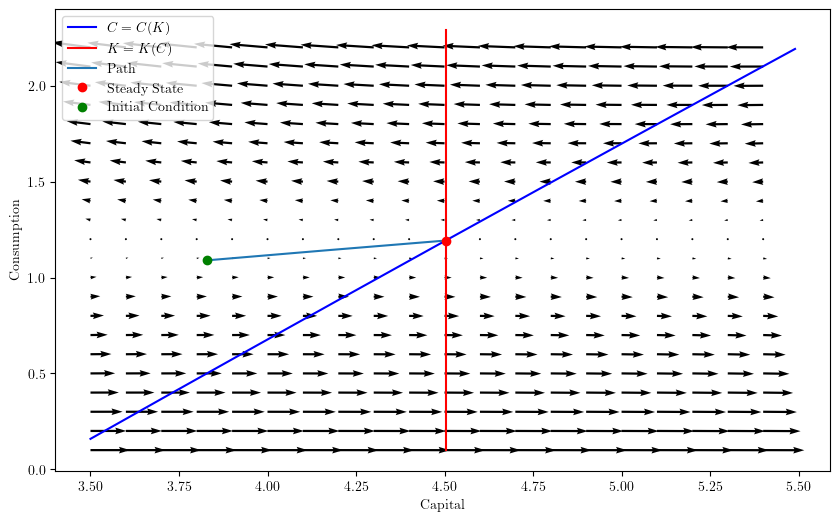
\includegraphics[width=10cm]{macro_hw1_code/phase_diagram.png}
		\caption{Phase Diagram}
		\label{fig:phase_diagram}
	\end{figure} 
	\item As agents get more impatient, they want to increase consumption in the current period rather than save capital for later. This leads, when they are significantly impatient, to no convergence. If there is convergence, it actually converges faster the more impatient agents are. A plot of the iterations to convergence on the value of $\beta$ is Figure~\ref{fig:iters}. I discretized $\beta$ from $0.9$ to $0.98$. The empty values are where the model did not converge (including everything from 0.9 to 0.96). Convergence was slightly faster for some values just below the previous rate, but increased when it was far below.
	\begin{figure}[H]
		\centering
		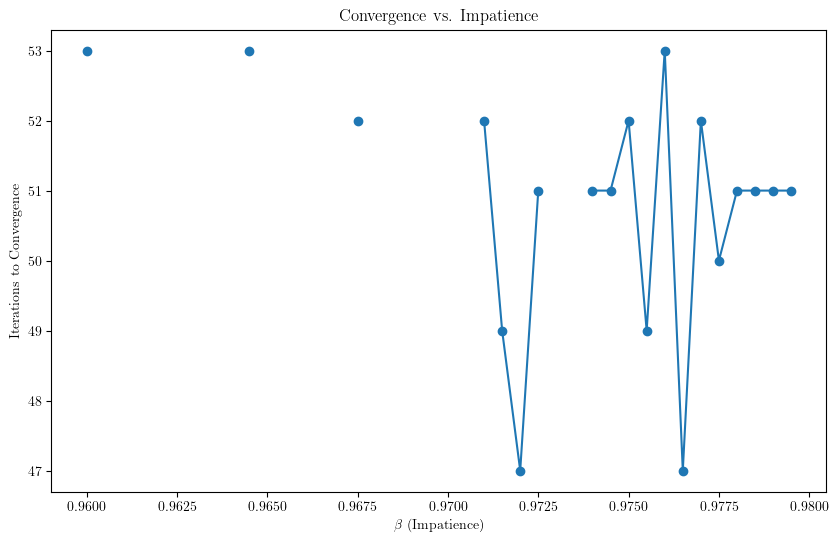
\includegraphics[width=10cm]{macro_hw1_code/iters.png}
		\caption{Convergence on Impatience}
		\label{fig:iters}
	\end{figure}
	\item Similarly to class, we can write the one-sector growth model in recursive formulation as follows: \[V(k) = \max_{(c,k') \in \Gamma(k)} \frac{c^{1-\sigma}}{1-\sigma} + \beta V(k')\]where\[\Gamma(k) = \{(c,k') : c \ge 0, k' \ge 0, c + k' \le f(k) + (1-\delta)k\}\]To perform the value function iteration, we guess an initial value function $V_0 = 0$, and discretize the capital and consumption spaces around the steady states. We then iteratively guess value functions until we converge to the optimal policy function $k'(k)$ and value function $V(k)$. The attained optimal capital accumulation function and the Euler residuals are in Figure~\ref{fig:vfi_plots}.
	\begin{figure}[H]
		\centering
		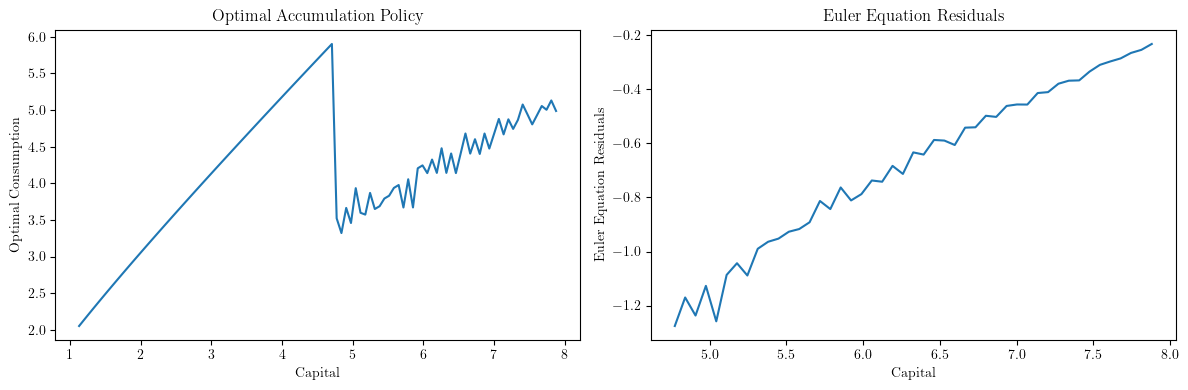
\includegraphics[width=16cm]{macro_hw1_code/value_function_iteration.png}
		\caption{Optimal Accumulation Policy and Euler Equation Residuals}
		\label{fig:vfi_plots}
	\end{figure}
	\item The policy function path and the shooting method path are in Figure~\ref{fig:transition_paths}, with the policy function path in blue, the shooting method path in orange, and the steady state in red. As we can see, the policy function path oscillates around the steady state significantly more than the shooting method path.
	\begin{figure}[H]
		\centering
		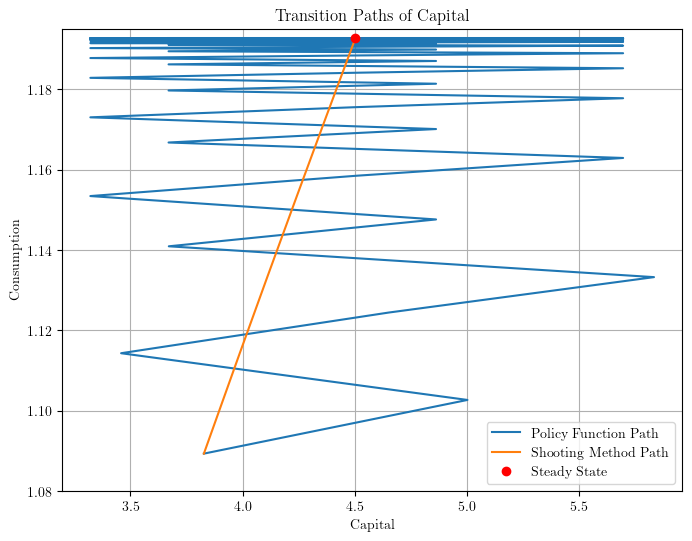
\includegraphics[width=10cm]{macro_hw1_code/transition_paths.png}
		\caption{Transition Paths of Capital}
		\label{fig:transition_paths}
	\end{figure}
\end{enumerate}

My code for this problem is:

\lstinputlisting[language=Python]{/Users/gabesekeres/Dropbox/Notes/Cornell_Notes/01_Spring_2025/6140_Macroeconomics/Completed_Homeworks/macro_hw1_code/main.py}














































\end{document}